\documentclass[10pt]{article}
\usepackage[pdftex]{graphicx}
\graphicspath{{./images/}}
\usepackage{amsmath,amssymb}
\DeclareMathOperator*{\argmin}{\arg\!\min}
\usepackage{dirtytalk}
\usepackage{xcolor}
\usepackage{hyperref}
\hypersetup{
    colorlinks,
    linkcolor={red!50!black},
    citecolor={blue!50!black},
    urlcolor={blue!80!black}
}
\usepackage[skip=10pt plus1pt, indent=40pt]{parskip}
\usepackage{../common_styles/csagh}


\begin{document}
\begin{opening}
  \title{Linear regression with Python}
  \author[Universidad Autónoma de Nuevo León, San Nicolás de los Garza, aldo.hernandezt@uanl.edu.mx]{Aldo Hernández}

  \keywords{...}
  \begin{abstract}
    %heh%
  \end{abstract}

  \keywords{linear regression, python, model, tendency, machine learning}
\end{opening}

\section{Introduction}
Linear regression is a fairly common algorithm in statistics and machine learning to make predictions and show tendencies given a certain dataset. This algorithm \textit{finds} a straight line---also known as "fitting" a line---that indicates a tendency and makes predictions from it \cite{aprendeML}. This model is widely used as an activation function on neural networks for some specific tasks but it is required to be combined with other non-linear functions in order to recognize more complex patterns. \par
The straight line is represented as
\begin{equation*}
    h_{w}(x) = w_{1}x + w_{0}
\end{equation*}
Where $\begin{bmatrix} w_{0} & w_{1} \end{bmatrix}$ is known as the weight vector and are the coefficients to be learned---or "found"---. The task of finding the $h_{w}$ that fits best this data is called \textbf{linear regression}. To do this, we simply have to find the values of the weight vector that minimize the empirical loss. It is traditional to use the squared loss function $L_{2}$ summed all over the training set \cite{ai} \par
\begin{equation*}
    Loss(h_{w}) = \sum_{j=1}^{N}L_{2}(y_{j}, h_{w}(x_{j})) = \sum_{j=1}^{N}(y_{j} - h_{w}(x_{j}))^{2} = \sum_{j=1}^{N}(y_{j} - (w_{1}x_{j} + w_{0}))^{2}
\end{equation*}

We would like to find $\textbf{w*} = \argmin_{w} Loss(h_{w})$. To minimize this function we have to partially differentiate with respect to each weight and set those equations to zero, since they will be at a minimum when their partial derivative is zero: \par
\begin{equation*}
    \begin{cases}
        \frac{\partial}{\partial w_{0}} \sum_{j=1}^{N}(y_{j} - (w_{1}x_{j} + w_{0}))^{2} = 0 \\
        \frac{\partial}{\partial w_{1}} \sum_{j=1}^{N}(y_{j} - (w_{1}x_{j} + w_{0}))^{2} = 0
    \end{cases} 
\end{equation*}

This equation system has a unique solution for the weight vector given by: \par
\begin{equation*}
    w_{1} = \frac{N(\Sigma x_{j}y_{j}) - (\Sigma x_{j})(\Sigma y_{j})}{N(\Sigma x_{j}^{2}) - (\Sigma x_{j})^2} \,;\, w_{0} = \frac{\Sigma y_{j} - w_{1}\Sigma x_{j}}{N}
\end{equation*}

Since in this way of learning we want to minimize a loss, it is useful to have a mental picture of what is going on in the \textbf{weight space}---the space defined by all possible settings of the weights. For univariate linear regression, this space is two-dimensional, hence we can graph the loss as a function of $w_{0}$ and $w_{1}$ in a 3D plot as seen in figure \ref{fig:loss_function}. \par

\newpage

\begin{figure}[h]
    \centering
    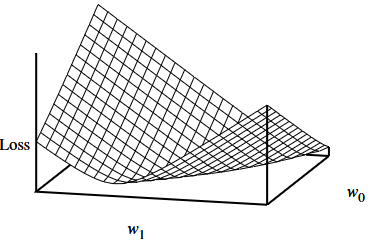
\includegraphics[width=60mm]{2025-03-26-09-24-32.png}
    \caption{Example loss function taken from \cite{ai}}
    \label{fig:loss_function}
\end{figure}

As we can see, this function is \textbf{convex}, and this is true for \textit{every} linear regression problem with an $L_{2}$ loss function, it also implies that there are no \textit{local minima}. \cite{ai} \par

When applying this concept in machine learning, it is important to note that we need a \textbf{learning rate} $\alpha$---also known as step size---that can be a fixed constant or decay over time, in purpose of minimizing the $Loss$ function. \par

For $N$ training samples, we want to minimize the sum of individual losses for each pair in the set, so we have
\begin{equation*}
    w_{0} \leftarrow w_{0} + \alpha\sum_{j}(y_{j} - h_{w}(x_{j})); \,\,\, w_{1} \leftarrow w_{1} + \alpha\sum_{j}(y_{j} - h_{w}(x_{j})) \times x_{j}
\end{equation*}

These updates constitute the \textbf{batch gradient descent} learning rule for univariate linear regression \cite{ai} that is a machine learning algorithm that uses the whole training dataset to optimize a training model. Convergence to a unique global minimum is guaranteed---as long as $\alpha$ is small enough---but may be vary slow since we have to cycle through all the training data for every step, and there may be a lot of steps \cite{ai}. This is essentially what linear regression models use to fit best the training dataset.

\newpage

\section{Methodology}
\subsection{Before typing code}
Before we start the activity, we must download the following \href{http://www.aprendemachinelearning.com/articulos_ml/}{.csv file} \cite{aprendeML} to use the same dataset. Also, we have to import the following Python packages:
\begin{itemize}
  \item Numpy
  \item Pandas
  \item Matplotlib
  \item Scikit-learn
\end{itemize}
After doing this, we are ready to import all of the needed packages to our Python main file: \par
As the reader can see, we also made some specific configuration for the program plots, such as size (in line 4) and style (in line 5); this may be changed according to the reader's preferences.

\subsection{Data processing}
Next, we will read the data from the .csv file using pandas to transform it into a dataframe. This is necessary since it will help us to easily remove all the columns that we will not use for the analysis, as shown in the figure: \par

\subsection{Filtering data}
Now that we have all of our essential data, we need to filter it in order to remove random anomalies in the dataset. In order to do this, we will take a look into the dataset information with the data.describe() method, but only to our two main columns:

\begin{table}[!ht]
  \centering
  \caption{Column information}
  \label{col_info}
    \begin{tabular}{|c|c|c|}
      \hline
       & Word count & \# Shares \\
      \hline
      Count & 161 & 161 \\
      \hline
      Mean & 1808.26 & 27948.348 \\
      \hline
      Std & 1141.919 & 43408.007 \\
      \hline
    \end{tabular}
\end{table}

As we can see in table \ref{col_info}, there are no null values in the columns, and our values are not very concentrated. Since we can't do really much with this information, we will graph a histogram to see where our data is really concentrated using the hist() method right after dropping the unnecessary columns: \par

Thanks to these graphics, we can now filter the data to remove anomalies. To do so, we will simply remove all data with more than 3500 words and data with more than 80000 shares with the following code: \par

We also colored data with orange if they are over the word count mean, or blue otherwise.

\subsection{Creating a new dataframe}
To create our multiple regression model, we will have to create a new dataframe with the columns that we will use as inputs. In this case, we will keep word count, but the other column will be the sum of links, comments, and images or videos. \par

We then create our training set as a NumPy array for $x$, $y$, and $z$, which are our 3-tuples $(x_{1}, y_{1}, z_{1})$

Finally, we create our model and fit it to the training data.

The reader may notice that we also print the coefficients $\left\{\beta_{0}, \beta_{1}, \beta_{2}\right\}$ of the linear function used for the model and some metrics to check the effectiveness of the model. These metrics are the \textit{Mean Squared Error}, and the \textit{Variance score}, where in ideal cases the MSE should be low and the variance score near one, which is not the case.

\subsection{Making a 3D graph with Matplotlib.pyplot}
Finally, we create a 3D plot using our new dataframe. We will start by creating a meshgrid where all of our $x$ and $y$ data will be distributed, and then make all of our plot values of a certain color (blue if from original set, red if it comes from a prediction using the training set). \par

The reader may wonder why the plot contains a big 2D plane, and it is as simple as that a line in 2D is a plane in 3D. With that stated, it is quite easy to visualize that said plane is our model, represented by the linear function
\begin{equation*}
  z = 21140.97 + 0.493x + 289.3253y
\end{equation*}

\section{Results}
Even though our model is not trustworthy, we can still make some predictions with it. For example, let's suppose we have an article with 2000 words, 10 links, 4 comments, and 6 images, according to our model, we would have around 27913 shares:
\begin{equation*}
  z = 21140.97 + 0.493(2000) + 289.3253(10+4+6) \approx 27913
\end{equation*}

\section{Conclusions}
Guided by the used metrics, it turned out our model was not trustworthy given the dataset. Although it seems like a failure, the model helped to find a tendency: the more words, links, comments, and images an article has, the more shares it will have. Of course it is not as simple as that, but given these inputs, the model suggests that this is true. We could prove it by reducing dimensions using an algorithm like Principal Component Analysis, but that is out of the purpose of this article. \par
Therefore, we conclude that the model is not suitable for small and dispersed datasets since it will probably lead to an underfitted model that will make bad predictions, but it remains useful to find a tendency early on during a larger investigation.

\bibliographystyle{../common_styles/cs-agh}
\bibliography{act9_bibliography}

\end{document}